\documentclass[11pt,class=report,crop=false]{standalone}
\usepackage[screen]{../python}

\begin{document}


%====================================================================
\chapitre{Ramsey graphs and combinatorics}
%====================================================================

\objectifs{You will see that a very simple problem, which concerns the relationships between only six people, will require a lot of calculations to be solved.}

\begin{center}
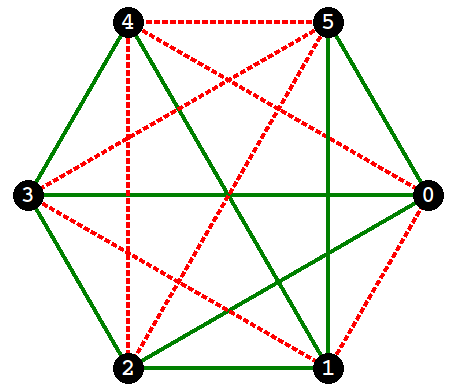
\includegraphics[scale=\myscale,scale=0.4]{screen-ramsey-1d}
\end{center} 

\index{graph}


%%%%%%%%%%%%%%%%%%%%%%%%%%%%%%%%%%%%%%%%%%%%%%%%%%%%%%%%%%%%%%%%
%%%%%%%%%%%%%%%%%%%%%%%%%%%%%%%%%%%%%%%%%%%%%%%%%%%%%%%%%%%%%%%%

\begin{cours}[Ramsey's problem]

\objectifs{Proposition. In a group of $6$ people, there is always $3$ friends (the three know each other two by two) or $3$ foreigners (all three are strangers to each other).}

The purpose of this chapter is to have the computer demonstrate this statement. For that we will model the problem by graphs, then we will check the statement for each of the $32\,768$ possible graphs.

\bigskip 

We consider $n$ people. For two of them, either they know each other (they are friends) or they do not know each other (they are strangers to each other). We schematize this by a graph:
\begin{itemize}
  \item a person is represented by a vertex (numbered from $0$ to $n-1$);
  \item if two people are friends, the corresponding vertices are connected by a green solid edge;
  \item otherwise (they are strangers), the corresponding vertices are connected by a red dotted edge. 
\end{itemize}

The graph below means that $0$ is friend with $2$; $1$ is friend with $3$. The other pairs don't know each other.
\myfigure{0.8}{
  \tikzinput{fig-ramsey-0a}
}

A graph checks the Ramsey problem, if there are among its vertices, either $3$ friends, or either $3$ foreigners.
\myfigure{0.4}{
  \tikzinput{fig-ramsey-0b}
}

Here is an example of $5$ peoples that verify the statement: there is group of $3$ strangers (the $0$, $2$ and $4$ vertices), even if there is no group of three friends.

\myfigure{0.5}{
  \tikzinput{fig-ramsey-0c}
}
\end{cours}


\begin{cours}[Model]


\objectifs{We model a graph by an array, containing $0$ and $1$.}

Let be a graph with $n$ vertices, numbered from $0$ to $n-1$.
The \defi{array of the graph} is a table of size $n \times n$ in which we place a $1$ in position $(i,j)$ if the vertices $i$ and $j$ are connected by an edge, otherwise we place a $0$.

\bigskip
First example below: the vertices $0$ and $2$ are friends (because they are connected by a green edge) so the table contains a $1$ in position $(0,2)$ and also in $(2,0)$. Similarly $1$ and $3$ are friends, so the table contains a $1$ in position $(1,3)$ and $(3,1)$. The rest of the table contains $0$.

\myfigure{0.7}{
  \tikzinput{fig-ramsey-1a}
}

Here is a more complicated graph and its array:
\myfigure{0.7}{
  \tikzinput{fig-ramsey-1c}
}

\end{cours}



%%%%%%%%%%%%%%%%%%%%%%%%%%%%%%%%%%%%%%%%%%%%%%%%%%%%%%%%%%%%%%%%
% Activity 1
%%%%%%%%%%%%%%%%%%%%%%%%%%%%%%%%%%%%%%%%%%%%%%%%%%%%%%%%%%%%%%%%

\begin{activite}[Build graphs]

\objectifs{Goal: define graphs and test if three given vertices are friends.}


\begin{center}
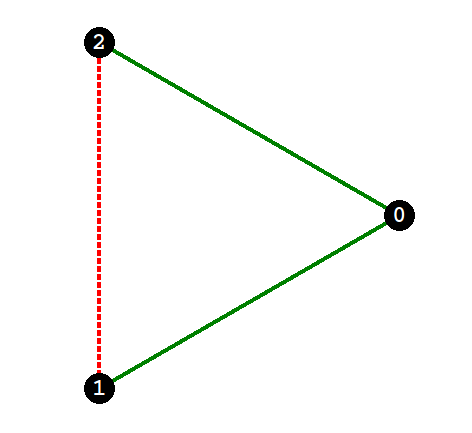
\includegraphics[scale=\myscale,height=5cm]{screen-ramsey-1a}\quad
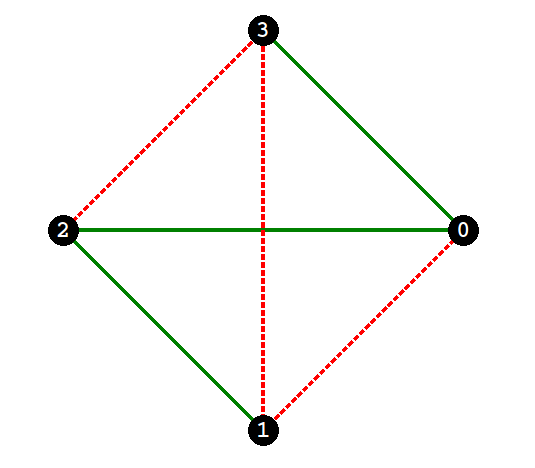
\includegraphics[scale=\myscale,height=5cm]{screen-ramsey-1b}
\end{center} 
\begin{center}
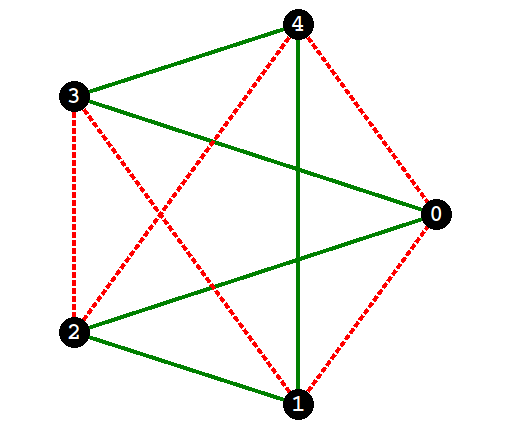
\includegraphics[scale=\myscale,height=5cm]{screen-ramsey-1c}\quad
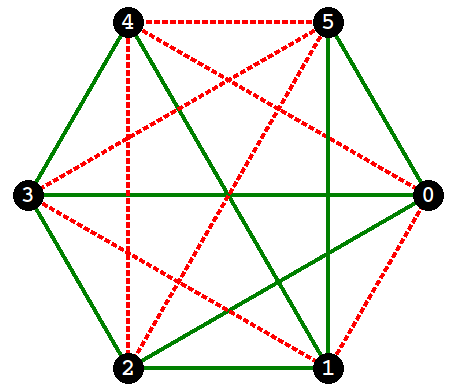
\includegraphics[scale=\myscale,height=5cm]{screen-ramsey-1d}
\end{center} 


\begin{enumerate}
  \item Define the graph array for the four examples above.
  You can start by initializing the array with   
  \mycenterline{\ci{array = [[0 for j in range(n)] for i in range(n)]}}
  
  Then add commands: 
  \mycenterline{\ci{array[i][j] = 1} \quad and \quad \ci{array[j][i] = 1}}
  
  Don't forget that if the $i$ vertex is connected to the $j$ vertex by an edge, then you have to put a $1$ in position $(i,j)$ but also in position $(j,i)$. 
  
  \item Define a function \ci{print_graph(array)} that allows you to display on the screen the table of a graph.
  Thus the third example above (with $n=5$) should be displayed as follows:
\begin{center}
\ci{0 0 1 1 0}\\
\ci{0 0 1 0 1}\\
\ci{1 1 0 0 0}\\
\ci{1 0 0 0 1}\\
\ci{0 1 0 1 0}\\
\end{center}

  \item We set three vertices $i$, $j$, $k$ of a graph. Write a function \ci{have_3_fix_friends(array,i,j,k)} that tests if the vertices $i$, $j$, $k$ are three friends (the function returns \og{}True\fg{} or \og{}False\fg{}). Do the same work with a \ci{have_3_fix_strangers(array,i,j,k)} function to find out if these vertices are strangers.
  
Find by hand on the fourth example, three friend or foreign vertices and check your answer using the functions you have just defined on these vertices.

\end{enumerate}   
     
\end{activite}


%%%%%%%%%%%%%%%%%%%%%%%%%%%%%%%%%%%%%%%%%%%%%%%%%%%%%%%%%%%%%%%%
% Activity 2
%%%%%%%%%%%%%%%%%%%%%%%%%%%%%%%%%%%%%%%%%%%%%%%%%%%%%%%%%%%%%%%%

\begin{activite}[Draw nice graphs]

\objectifs{Goal: draw a graph! Optional activity. }

\begin{center}
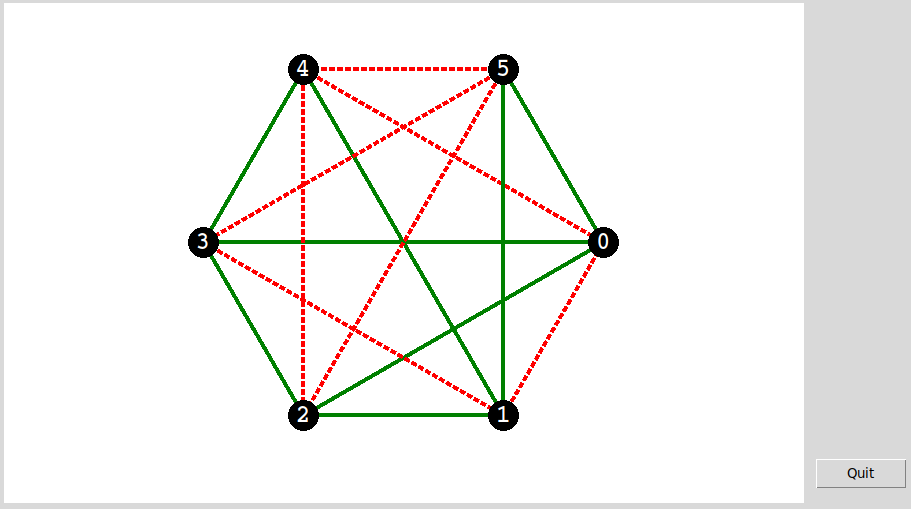
\includegraphics[scale=\myscale,scale=0.4]{screen-ramsey-2-en}
\end{center}


Program the graphical display of a graph by a function \ci{display_graph(array)}.
     
\bigskip
     
\emph{Hints.} This activity is not necessary for the next steps, it just helps to visualize the graphs. It is necessary to use the module \ci{tkinter} and the functions \ci{create_line()}, \ci{create_oval()} and possibly \ci{create_text()}. 
% See previous sheets.

The most delicate point is to obtain the coordinates of the vertices. You will need the sine and cosine functions (available in the module \ci{math}).
The coordinates $(x_i,y_i)$ of the vertex number $i$ of a graph with $n$ elements can be calculated by the formulas :
$$x_i = r \cos\left(\frac{2 i \pi}{n}\right) \qquad \text{ and } \qquad y_i = r\sin\left(\frac{2 i \pi}{n}\right).$$

These vertices are located on the circle of radius $r$, centered at $(0,0)$. 
You will have to choose $r$ large enough (for example $r=200$) and shift the circle to display it on the screen.


\myfigure{0.7}{
  \tikzinput{fig-ramsey-2}
}
\end{activite}

%%%%%%%%%%%%%%%%%%%%%%%%%%%%%%%%%%%%%%%%%%%%%%%%%%%%%%%%%%%%%%%%
% Activity 3
%%%%%%%%%%%%%%%%%%%%%%%%%%%%%%%%%%%%%%%%%%%%%%%%%%%%%%%%%%%%%%%%

\begin{activite}[Binary notation with zero-padding]

\objectifs{Goal: convert an integer to binary notation with possible leading zeros.}

\index{binary}


Program an \ci{integer_to_binary(p,n)} function that displays the binary notation of an integer $p$ on $n$ bits. The result is a list of $0$ and $1$.

\bigskip

Example.
\begin{itemize}
  \item The binary notation of $p=37$ is $1.0.0.1.0.1$. If you want its binary notation on $n=8$ bits you have to add two $0$ in front of it: $0.0.1.0.0.1.0.1$. 
  \item So the result of the command \ci{integer_to_binary(37,8)} must be \ci{[0, 0, 1, 0, 0, 1, 0, 1]}.
  \item The command \ci{integer_to_binary(37,10)} returns the binary notation of $37$ on $10$ bits: \ci{[0, 0, 0, 0, 1, 0, 0, 1, 0, 1]}.
\end{itemize}

\bigskip

\emph{Hints.}
\begin{itemize}
  \item You can use the command \ci{bin(p)}.
  \item The command \ci{list(mystring)}\index{list@\ci{list}}\index{string} returns the list of characters making up \ci{mystring}.
  \item Attention! We want a list of integers \ci{0} or \ci{1}, not of characters \ci{'0'} or \ci{'1'}. The command \ci{int('0')} returns \ci{0} and \ci{int('1')} returns \ci{1}.
  
  \item \ci{mylist = mylist + [element]} adds an item at the end of the list, while \ci{mylist = [element] + mylist} adds the item at the beginning of the list.
\end{itemize} 
  
\end{activite}


%%%%%%%%%%%%%%%%%%%%%%%%%%%%%%%%%%%%%%%%%%%%%%%%%%%%%%%%%%%%%%%%
% Activity 4
%%%%%%%%%%%%%%%%%%%%%%%%%%%%%%%%%%%%%%%%%%%%%%%%%%%%%%%%%%%%%%%%

\begin{cours}[Subsets]

Let $E_n = \{0,1,2,\ldots,n-1\}$ be the set of all integers from $0$ to $n-1$. The set $E_n$ therefore contains $n$ elements.
For example $E_3 = \{ 0,1,2 \}$, $E_4 = \{ 0,1,2,3 \}$\ldots

\bigskip

\textbf{Subsets.}

What are the subsets of $E_n$? For example there are $8$ subsets of $E_3$, these are:
    \begin{itemize}
      \item the subset $\{0\}$ composed of the single element $0$;
      \item the subset $\{1\}$ composed of the single element $1$;      
      \item the subset $\{2\}$ composed of the single element $2$; 
      \item the subset $\{0,1\}$ composed of the element $0$ and the element $1$;           
      \item the subset $\{0,2\}$;
      \item the subset $\{1,2\}$; 
      \item the subset $\{0, 1,2\}$ composed of all elements;
      \item and the empty set $\varnothing$ which contains no elements!    
    \end{itemize} 

\medskip

\textbf{Proposition.} The set $E_n$ contains $2^n$ subsets.

\medskip

For example $E_4 = \{ 0,1,2,3 \}$ has $2^4 = 16$ possible subsets. Have fun finding them all! For $E_6$ there is $2^6 = 64$ possible subsets.

\bigskip

\textbf{Subsets of fixed cardinal.}

We are only looking for subsets with a fixed number $k$ of elements.

Examples:
\begin{itemize}
  \item For $n = 3$ and $k = 2$, the subsets having two elements and contained in $E_3 = \{ 0,1,2 \}$ are the three pairs: $\{0,1\}$, $\{0,2\}$, $\{1,2\}$.

  \item For $n = 5$ and $k = 3$, the subsets having three elements and contained in $E_5 = \{ 0,1,2,3,4 \}$ are the $10$ triples:
  $\{0, 1, 2\}$, $\{0, 1, 3\}$, $\{0, 2, 3\}$, $\{1, 2, 3\}$, $\{0, 1, 4\}$, $\{0, 2, 4\}$, $\{1, 2, 4\}$, $\{0, 3, 4\}$, $\{1, 3, 4\}$, $\{2, 3, 4\}$.
  
\end{itemize}

\end{cours}


\begin{activite}[Subsets]

\objectifs{Goal: generate all subsets to test all triples of vertices. For this we will use binary notation.}

Here is how we associate to each integer $p$ verifying $0 \le p < 2^n$ a subset of $E_n = \{0,1,\ldots, n-1\}$.

Let's start with an example, with $n = 6$ and $p=26$:
\begin{itemize}
  \item the binary notation of $p=26$ on $n=6$ bits is 
  \ci[0,1,1,0,1,0];
  \item there are $1$ at ranks $1$, $2$ and $4$ (starting at rank $0$ on the left);
  \item the associated subset is then $\{1,2,4\}$.
\end{itemize}


\myfigure{0.7}{
  \tikzinput{fig-ramsey-4a}
}


\bigskip

Other examples.
\begin{itemize}
  \item With $n = 8$ and $p = 57$ whose binary notation on $8$ bits is \ci{[0,0,1,1,1,0,0,1]}, the associated subset corresponds to the ranks $2,3,4,7$, so it is $\{2,3,4,7\}$.
  
  \smallskip
  
\myfigure{0.6}{
  \tikzinput{fig-ramsey-4b}
}  

  
  \item With $p=0$, the binary notation is only formed of $0$, the associated subset is the empty set.
  \item With $p = 2^n - 1$, the binary notation is full of $1$, the associated subset is the whole set $E_n = \{0,1,\ldots, n-1\}$ itself.
\end{itemize}

\bigskip

We model a set as a list of elements.
For example:
\begin{itemize}
  \item The set $E_4$ is for us the list \ci{[0,1,2,3]}.
  \item A subset of $E_4$ is for example the pair \ci{[1,3]}.
  \item The empty set is represented by the empty list \ci{[]}.
\end{itemize}



\begin{enumerate}
  \item Program a function \ci{subsets(n)} which returns the list of all possible subsets of $E_n =  \{0,1,2,\ldots,n-1\}$.
  For example, with $n=3$, \ci{subsets(n)} returns the list (which itself contains lists):
\mycenterline{\ci{[ [], [2], [1], [1, 2], [0], [0, 2], [0, 1], [0, 1, 2]  ]}}

That is to say the $8$ subsets (starting with the empty set):
$$\varnothing \quad \{2\}\quad \{1\}\quad \{1,2\}\quad \{0\}\quad \{0,2\}\quad \{0,1\}\quad \{0,1,2\}.$$

\emph{Hint.} To test your program, check that the returned list contains $2^n$ subsets.

  \item Deduce a function \ci{fix_subsets(n,k)} from it that returns only subsets of $E_n$ with $k$ elements.
  
 For example, for $n=3$ and $k=2$, \ci{fix_subsets(n,k)} returns the list of pairs:
\mycenterline{\ci{[ [0, 1], [0, 2], [1, 2] ]}}
 
Test your program:
\begin{itemize}
  \item For $n=4$ and $k=3$, the list returned by \ci{fix_subsets(n,k)} contains $4$ triples.
  \item For $n=5$ and $k=3$, there are $10$ triples possible.
  \item For $n=10$ and $k=4$, there are $210$ possible subsets!
\end{itemize}

\end{enumerate}  


In the following we will use mainly subsets having $3$ elements.
In particular, for $n=6$, there are $20$ triples included in $\{0,1,2,3,4,5\}$:
\begin{center}
\ci{[[3, 4, 5], [2, 4, 5], [2, 3, 5], [2, 3, 4], [1, 4, 5], }
\ci{ [1, 3, 5], [1, 3, 4], [1, 2, 5], [1, 2, 4], [1, 2, 3],}
\ci{ [0, 4, 5], [0, 3, 5], [0, 3, 4], [0, 2, 5], [0, 2, 4], }
\ci{ [0, 2, 3], [0, 1, 5], [0, 1, 4], [0, 1, 3], [0, 1, 2]]}
\end{center}
   
\end{activite}

%%%%%%%%%%%%%%%%%%%%%%%%%%%%%%%%%%%%%%%%%%%%%%%%%%%%%%%%%%%%%%%%
% Activity 5
%%%%%%%%%%%%%%%%%%%%%%%%%%%%%%%%%%%%%%%%%%%%%%%%%%%%%%%%%%%%%%%%

\begin{activite}[Ramsey's theorem for $n=6$]

\objectifs{Goal: check that all graphs with $6$ vertices contain three friends or three strangers.}

\begin{enumerate}
  \item Program a function \ci{have_3(array)} that tests if a graph contains $3$ friends or $3$ foreigners. You must therefore call the functions \ci{have_3_fix_friends(array,i,j,k)} and \ci{have_3_fix_strangers(array,i,j,k)} of the first activity for all possible triples of vertices $(i,j,k)$.
 
 For the four examples of the first activity, only the fourth (with $6$ summits) checks the test.
  
  \item Program a function \ci{all_graphs(n)} that computes all possible graph arrays with $n$ vertices. There are $N = \frac{(n-1)n}{2}$ possible arrays. You can generate them by a method similar to the one for subsets:
  \begin{itemize}
    \item for each integer $p$ that verifies $0 \le p < 2^N$,
    \item calculate the binary notation of $p$ on $N$ bits,
    \item fill in the array element by element, with the $0$ and $1$ of the binary notation.
  \end{itemize}


\emph{Hints.}
To fill an array from a given binary notation of $p$ named \ci{binary_notation} (that is to say a list of $0$ and $1$), you can use a double loop like:

\begin{lstlisting}
for j in range(0,n):
    for i in range(j+1,n):
        b = binary_notation.pop()
        array[i][j] = b
        array[j][i] = b
\end{lstlisting}
  
Here is the principle of this loop that fills the part above the diagonal (and also the part below it by symmetry).
This loop takes the last bit of the list and places it on the first free box above the diagonal; then the penultimate bit is placed on the second free box\ldots; the first bit of the list fills the last free square.


 \myfigure{0.6}{
  \tikzinput{fig-ramsey-5}
} 
  
  \item Convert the previous function into a function \ci{test_all_graphs(n)}
which tests the conjecture \og{}there are three friends or three strangers\fg{} for all graphs with $n$ vertices.
You must find that:
\begin{itemize}
\item for $n=4$ and $n=5$ the guess is wrong. Give a graph having $4$ vertices (then $5$ vertices) that has neither $3$ friends, nor $3$ foreigners;
\item for $n=6$ let the computer check that, for each of the $N = 2^{\frac{5 \times 6}{2}} = 32\,768$ graphs with $6$ vertices, either it has $3$ friends or it has $3$ foreigners.
\end{itemize}
\end{enumerate}   
     
\end{activite}



\begin{activite}[To go further]

\objectifs{Goal: improve your program and prove other guesses. Optional activity. }

\begin{enumerate}
  \item Improve your program so that it checks the guess for $n=6$ in less than a second.
  
  
\emph{Ideas.}
  \begin{itemize}
    \item The list of triples must be generated once and for all at the beginning of the program (and not at each new graph).
    \item It is not necessary to generate a list of all possible graphs, then test them in a second step. It is better to generate one and then test it before moving on to the next.
    \item As soon as you find $3$ friends (or $3$ foreigners) it's won! Immediately stop the loop even if it means using the instruction \ci{break} and move to the next graph.
    \item You can only test the graphs that correspond to $p$ between $0$ and $2^{N}/2$ (because for the next $p$ it is like exchanging the green segments for red and vice versa).
  \end{itemize}
  
\medskip
  
  With these tips here are the calculation times you can expect:
  \begin{center}
  \begin{tabular}{|c|c|c|}
  \hline
  Number of vertices & Number of graphs & Approximate calculation time \\
  \hline\hline
  $n=6$ & 32\,768 & $< 1$ second \\
  $n=7$ & 2\,097\,152 & $< 1$ minute \\  
  $n=8$ & 268\,435\,456 & $< 1$ hour \\
  $n=9$ & 68\,719\,476\,476\,736 & $< 10$ days \\ 
  \hline
  \end{tabular} 
  \end{center}




 
  \item There is a more difficult statement. It is a question of finding out at which size $n$ a graph always contains either $4$ friends or $3$ foreigners. 
  Being $4$ friends means that two by two they are connected by a green segment, as below:
  \myfigure{1}{
  \tikzinput{fig-ramsey-6}
}  

  \begin{enumerate}
    \item Find graphs with $n=6$ (then $n=7$) vertices that do not check this statement.
    \item By searching a little with the machine find graphs with $8$ vertices that do not satisfy this statement.
    \item Prove that any graph having $9$ vertices contains $4$ friends or $3$ foreigners! 
     
  \emph{Hints.} It is necessary to test all the graphs corresponding to integers $p$ between $0$ and $2^N = 2^{\frac{8 \times 9}{2}} = 68\,719\,476\,736$. The total calculation time is about 20 days! You can share the calculations between several computers: one computer does the calculations for $0 \le p \le 1\,000\,000$, a second computer for $1\,000\,001 \le p \le 2\,000\,000$,\ldots
    
  \end{enumerate}
  
  \item 
  \begin{itemize}
    \item There are arguments to prove with pencil and paper that for $n=6$ there is always $3$ friends or $3$ foreigners. Look for such reasoning! With a little more effort, we can also prove that it is $n=9$ that answers the problem of $4$ friends/$3$ foreigners.
    
    \item We know how to prove that we need $n=18$ to always have $4$ friends or $4$ foreigners.
    
    \item However, no one in the world knows what the smallest $n$ is for the $5$ friends/$5$ foreigners problem!
  \end{itemize}

\end{enumerate}

\end{activite}


\end{document}
